\documentclass[main.tex]{subfiles}

\begin{document}

\section{Some other calculation}
This will probably be another calculation.



The full ggg splitting kernel is given by \autoref{eqn: medium_ggg_splittingfunction}.
To generate a random value from this function, we need to go back to the Metropolis-Hastings algorithm. 
For this we need a proportional dummy-function, we can use the simplified kernel given by (2.7) of EnergyFlowMedium \cite{Energy_flow_medium_cascade_2016}, 

\begin{equation}\label{eqn: medium_ggg_dummy_splittingfunction}
    \mathcal{K}(z) = \frac{1}{(z(1-z))^{3/2}}
\end{equation}

To be able to generate random momentum fractions for the branched parton, to be equal the distribution of \autoref{eqn: probability_density_for_splitting}, we need again to solve \autoref{eqn: energyfraction_function_R},

\begin{equation}\tag{\ref{eqn: energyfraction_function_R}}
    \mathcal{R} \cdot \int_\epsilon^{1-\epsilon} dz \, \hat{P}_{gg}(z) = \int_\epsilon^{y}dz \, \hat{P}_{gg}(z)
\end{equation}

using the dummy function given by \autoref{eqn: medium_ggg_dummy_splittingfunction}.

The integral can be generally shown to be, 

\begin{align}
    \int_a^b \frac{1}{(z(1-z))^{3/2}}dz &= \left[ \frac{4z-2}{\sqrt{-z(z-1)}} \right]_a^b
\end{align}

which means that we can evaluate \autoref{eqn: energyfraction_function_R} as,

\begin{align}
    \mathcal{R} \int_\epsilon^{1-\epsilon} dz \, \frac{1}{(z(1-z))^{3/2}} &= \int_\epsilon^{y} \frac{1}{(z(1-z))^{3/2}} \nonumber \\
    \mathcal{R} \left(  \frac{4(1-\epsilon)-2}{\sqrt{-(1-\epsilon)((1-\epsilon)-1)}} - \frac{4\epsilon-2}{\sqrt{-\epsilon(\epsilon-1)}} \right) &= \frac{4y-2}{\sqrt{-y(y-1)}} - \frac{4\epsilon-2}{\sqrt{-\epsilon(\epsilon-1)}} \nonumber\\
    \mathcal{R} \left(  \frac{2-4\epsilon}{\sqrt{\epsilon(1-\epsilon)}} - \frac{4\epsilon-2}{\sqrt{\epsilon(1-\epsilon)}} \right) &= \frac{4y-2}{\sqrt{-y(y-1)}} - \frac{4\epsilon-2}{\sqrt{-\epsilon(\epsilon-1)}} \nonumber\\
    \mathcal{R} \left(  \frac{4-8\epsilon}{\sqrt{\epsilon(1-\epsilon)}} \right) - \frac{2-4\epsilon}{\sqrt{\epsilon(1-\epsilon)}} &= \frac{4y-2}{\sqrt{-y(y-1)}} 
\end{align}

The term on the l.h.s can be written in terms of the integral again, 

\begin{equation}
    \mathcal{R} \left(  \frac{4-8\epsilon}{\sqrt{\epsilon(1-\epsilon)}} \right) + \frac{2-4\epsilon}{\sqrt{\epsilon(1-\epsilon)}}  = \int_\epsilon^{1-\epsilon} dz \cdot \left(\mathcal{R} - \frac{1}{2} \right) = a
\end{equation}

Inserting this \(a\), the remainder of the equation using Mathematica to obtain, 

\begin{align}\label{eqn: sampling_p_ggg_medium}
    y &= \frac{16 + a^2 \mp a \sqrt{16 + a^2}}{2 (16 + a^2)} \nonumber\\
    y &= \frac{1}{2} \mp \frac{a \sqrt{16 + a^2}}{2 (16 + a^2)} \nonumber\\
    y &= \frac{1}{2} \mp \frac{a }{2 \sqrt{16 + a^2}}
\end{align}

We now have a method for randomly drawing a sample from the dummy splitting function, and can follow the procedure of \autoref{sec: metropolis_hastings} to implement \autoref{eqn: sampling_p_ggg_medium} into a MH algorithm to draw samples from the full splitting function. The plots of the original histogram, and MH corrected histogram is given in \autoref{fig: MH_corrected_p_gg_medium_splitting}.

\begin{figure}[ht]
    \centering
    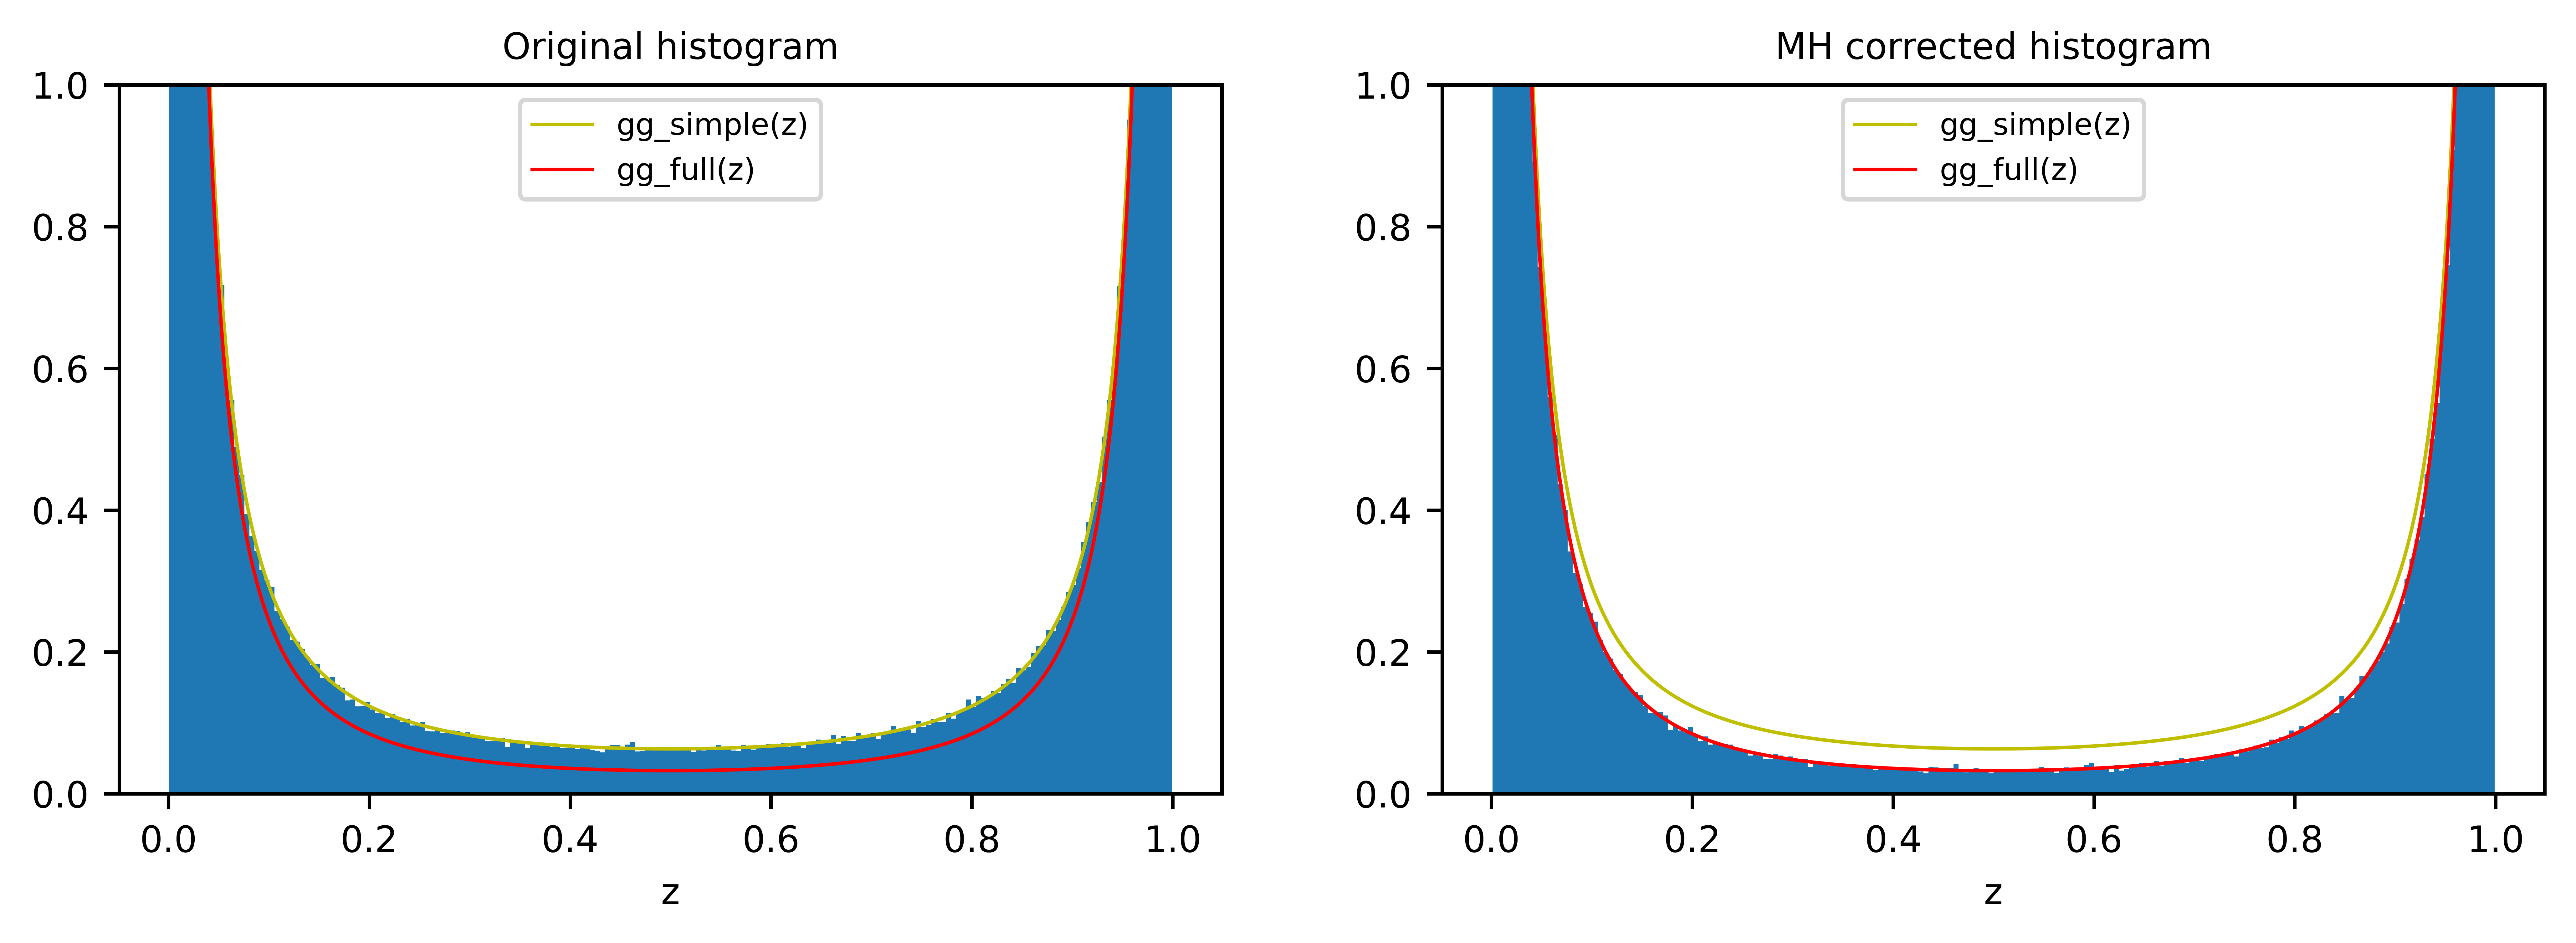
\includegraphics[width=14cm]{pictures/MH_plots/MH_medium_gg.png}
    \caption{Probability density of the medium \(\hat{P}_{gg}\) splitting function, compared to the histogram of the dummy splitting function, and the Metropolis-Hastings corrected results. Simulated with \(1,000,000\) points, and an acceptance rate of \(0.95\).}
    \label{fig: MH_corrected_p_gg_medium_splitting}
\end{figure}

\subsubsection{g-qq vertex in Medium}
Continuing now with the \(qg\) splitting function, \autoref{eqn: medium_qgg_splittingfunction}, 

\begin{equation}\tag{\ref{eqn: medium_qgg_splittingfunction}}
    \mathcal{K}_{qg}(z) = \frac{1}{2} \, 2\, N_f T_F \left(z^2 + (1-z)^2 \right) \, \sqrt{\frac{C_F - z(1-z) \, C_A}{z(1-z)}}
\end{equation}

With some inspiration from the previous section, we can propose the following dummy function,

\begin{equation}
    \mathcal{K}_{qg}(z) = \frac{1}{2} \, 2\, N_f T_F \frac{1}{\sqrt{z (1-z)}}
\end{equation}

The integral can be shown to be, 

\begin{align}
    \int_a^b \frac{1}{\sqrt{x(1-x)} } &= -2 sin^{-1}(\sqrt{1-x})
\end{align}

so when evaluating \autoref{eqn: energyfraction_function_R} we get,

\begin{align}
    \mathcal{R}\left( -2 sin^{-1}(\sqrt{\epsilon}) + 2 sin^{-1}(\sqrt{1-\epsilon})  \right) &= -2 sin^{-1}(\sqrt{1-y}) + 2 sin^{-1}(\sqrt{1-\epsilon}) \nonumber\\
    -\mathcal{R} \cdot 3.015080456 + 3.078336555 &= 2 sin^{-1}(\sqrt{1-y}) 
\end{align}

setting \(a = -\mathcal{R} \cdot 3.015080456 + 3.078336555\), and solving for y, 

\begin{align}\label{eqn: sampling_p_gqq_medium}
    y &= 1- \sqrt{sin\left(\frac{a}{2}\right)}
\end{align}

Using \autoref{eqn: sampling_p_gqq_medium} to sample values for the dummy function, we can run the MH algorithm as in previous sections and obtain \autoref{fig: MH_corrected_p_qg_medium_splitting}.

\begin{figure}[ht]
    \centering
    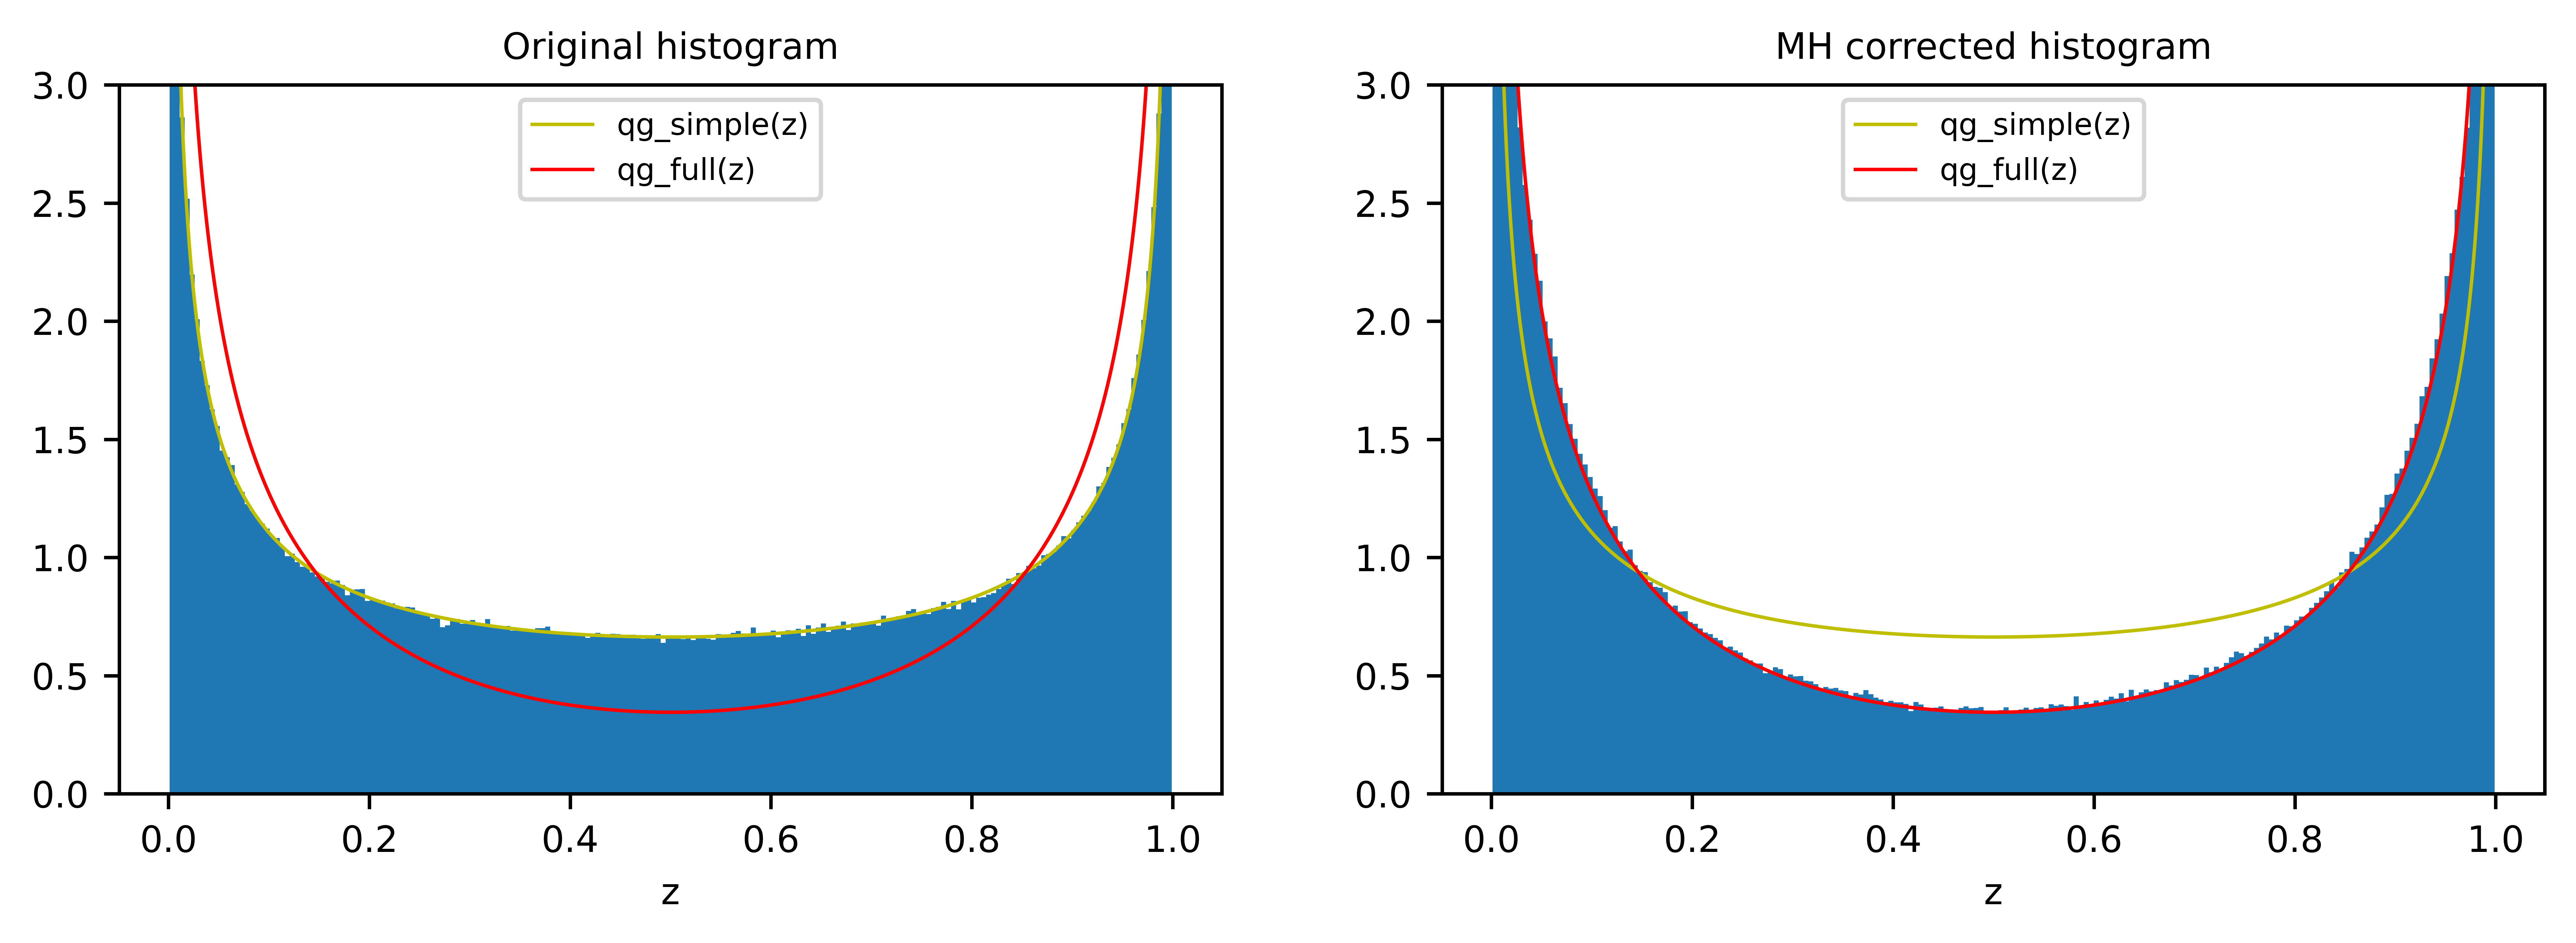
\includegraphics[width=14cm]{pictures/MH_plots/MH_medium_qg.png}
    \caption{Probability density of the medium \(\hat{P}_{qg}\) splitting function, compared to the histogram of the dummy splitting function, and the Metropolis-Hastings corrected results. Simulated with \(1,000,000\) points, and an acceptance rate of \(0.71\).}
    \label{fig: MH_corrected_p_qg_medium_splitting}
\end{figure}


\subsubsection{q-qg vertex in medium}
Finally we have the gq vertex, of \autoref{eqn: medium_qqg_splittingfunction}. 

\begin{equation}\tag{\ref{eqn: medium_qqg_splittingfunction}}
     \mathcal{K}_{qq}(z) = \frac{1}{2} \, C_F \, \frac{1+z^2}{1-z} \, \sqrt{\frac{z\, C_A + (1-z)^2 \, C_F}{z(1-z)}}
\end{equation}

From this we might try a dummy function such as, 

\begin{align}
    \mathcal{K}_{dummy} &= \frac{4}{z^{1/2} (1-z)^{3/2}}
\end{align}

The integral is, 

\begin{align}
    \int_a^b \frac{1}{(1-z)^{3/2}} dz &= \frac{8 \sqrt{z}}{\sqrt{1-z}}
\end{align}

And we can solve \autoref{eqn: energyfraction_function_R}, 

\begin{align}
    \mathcal{R} \cdot \left( \frac{8 \sqrt{1-\epsilon}}{\sqrt{\epsilon}} - \frac{8 \sqrt{\epsilon}}{\sqrt{1-\epsilon}} \right) &= \frac{8\sqrt{y}}{\sqrt{1-y}} - \frac{8\sqrt{\epsilon}}{\sqrt{1-\epsilon}} \nonumber\\
    \mathcal{R} \cdot 31.57532 + 0.03164  &= \frac{\sqrt{y}}{\sqrt{1-y}}
\end{align}

setting \(a = \mathcal{R} \cdot 31.57532 + 0.03164\), we can solve for \(y\)

\begin{align} \label{eqn: sampling_p_qqg_medium}
    y &= \frac{a^2}{1 + a^2} 
\end{align}

Implementing \autoref{eqn: sampling_p_qqg_medium} into the MH algorithm, we will obtain the following distribution given in \autoref{fig: MH_corrected_p_qq_medium_splitting}.

\begin{figure}[ht]
    \centering
    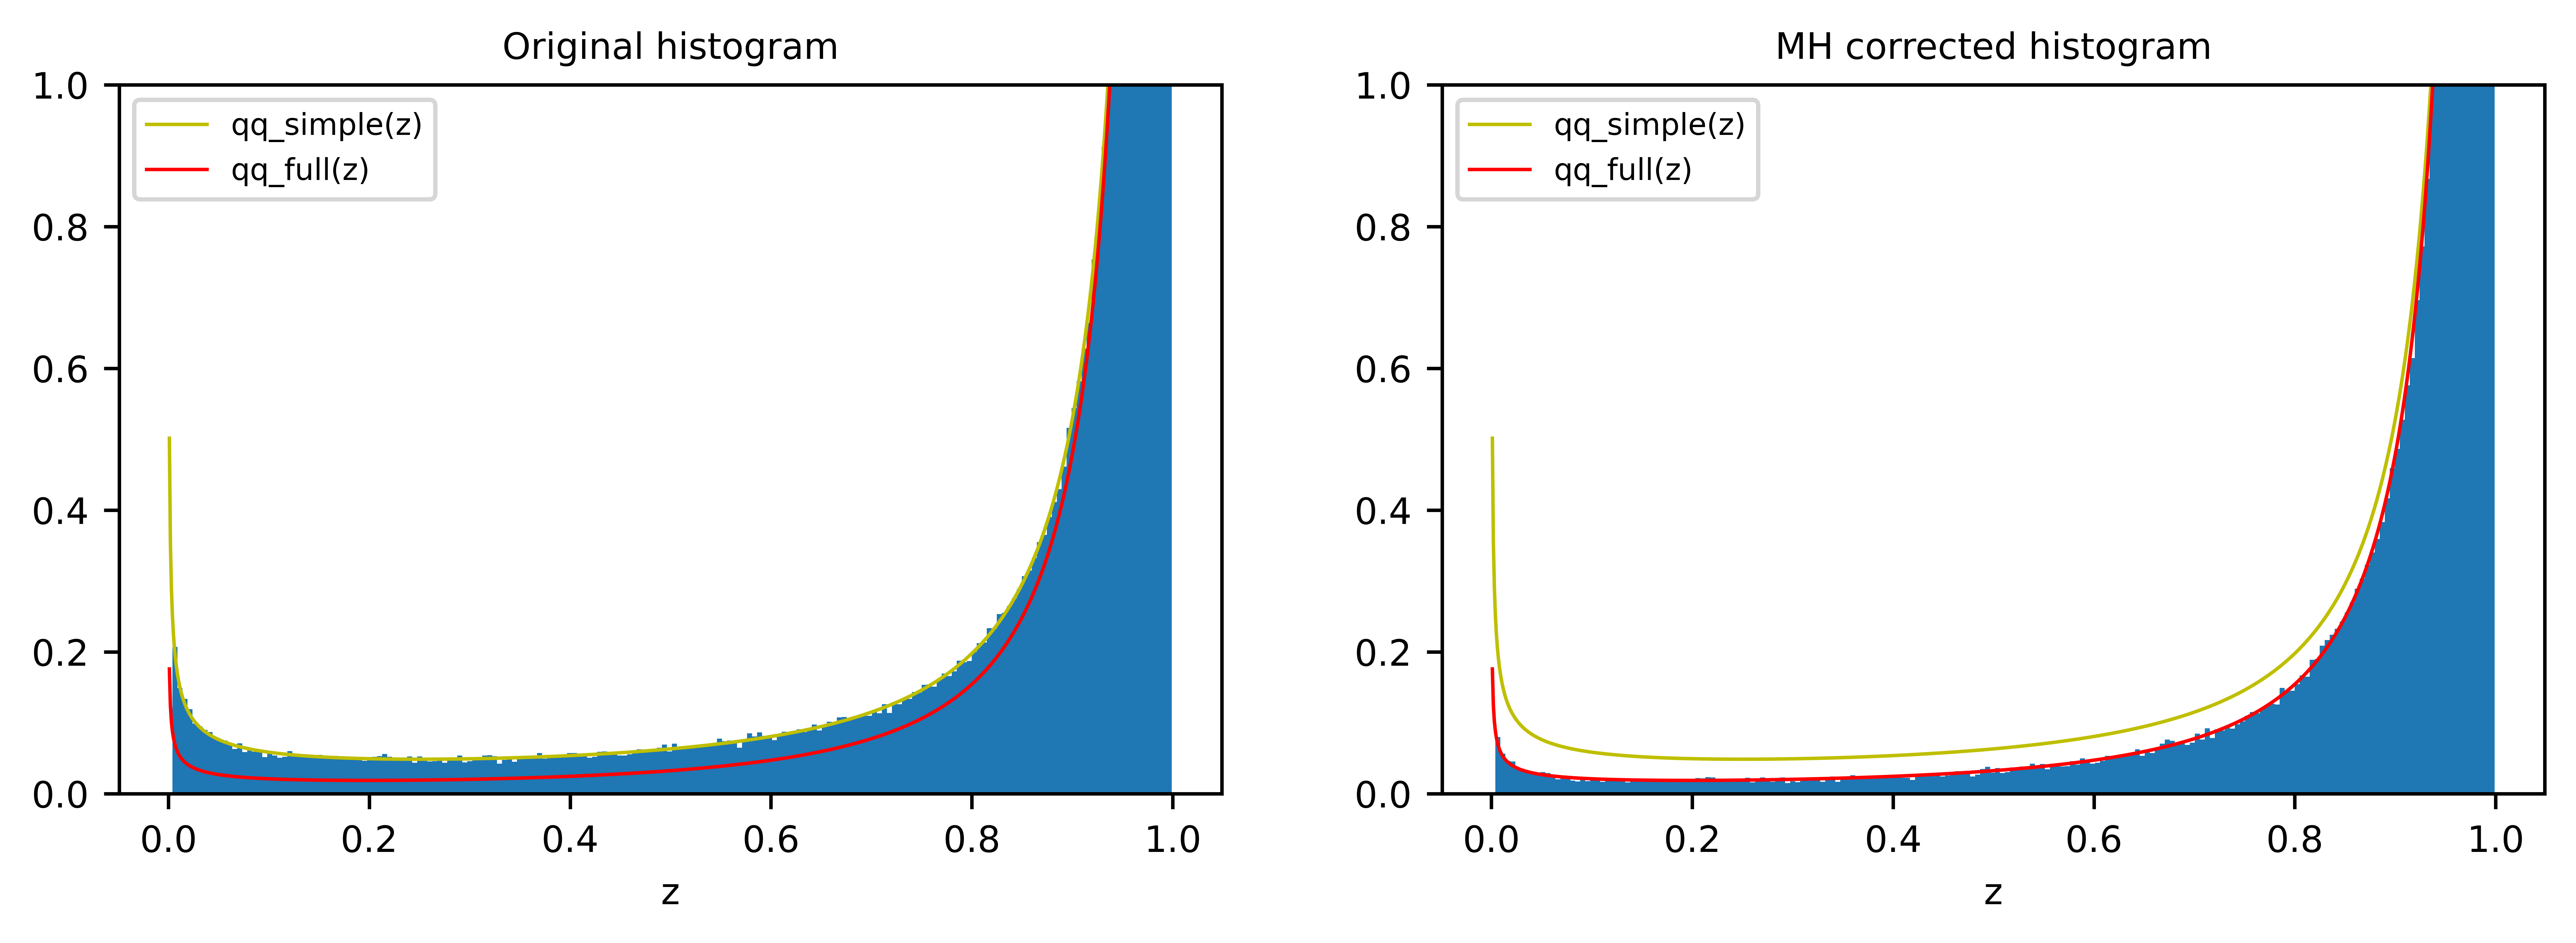
\includegraphics[width=14cm]{pictures/MH_plots/MH_medium_qq.png}
    \caption{Probability density of the medium \(\hat{P}_{qq}\) splitting function, compared to the histogram of the dummy splitting function, and the Metropolis-Hastings corrected results. Simulated with \(1,000,000\) points, and an acceptance rate of \(0.82\).}
    \label{fig: MH_corrected_p_qq_medium_splitting}
\end{figure}

\end{document}